% !TeX spellcheck = de_DE
\setcounter{section}{2}

\section{Wärmeübertragung}

\subsection{Wärmestrom und Wärmewiderstände}
	\setlength{\abovedisplayskip}{-20pt}
	\[ \arraycolsep=0.2em  \def\arraystretch{1.8}
	\begin{array}{r l l l l p{1em} l l}
		\Delta T & = R_{ges}\ \dot{Q}                          &                                         &                               &                   &  & R_{ges}        & = \dfrac{1}{k\ A_{wa}}     \\
		R        & = \dfrac{1}{k}                              & = R_{ges}\ A_{wa}                       & = \sum R_{einzel}             & = R_i + R_w + R_a &  & R_w            & = \sum_{N_w}^{j=1} R_{w,j} \\
		\dot{Q}  & = \dfrac{1}{R} A_{wa}\   \Delta T           & = k\ A_{wa}\ \Delta T                   &                               &                   &  & \Delta T       & = T_a - T_i                \\
		\dot{Q}  & = \dfrac{1}{R_i} A_{wa}\ \Delta T_i         & = \alpha_i\ A_{wa}\ \Delta T            &                               &                   &  & \Delta T_i     & = T_{wi} - T_i             \\
		\dot{Q}  & = \dfrac{1}{R_a} A_{wa}\ \Delta T_a         & = \alpha_a\ A_{wa}\ \Delta T            &                               &                   &  & \Delta T_a     & = T_a - T_{wa}             \\
		\dot{Q}  & = \dfrac{1}{R_{w,j}} A_{wa}\ \Delta T_{w,j} &                                         &                               &                   &  & \Delta T_{w,j} & = T_{w,j} - T_{w,j-1}      \\
		\dot{Q}  & = \dot{m}_H\ \abs{\Delta h_H}               & =  \dot{m}_H\ c_{p,H}\ \abs{\Delta T_H} & = \dot{W}_H\ \abs{\Delta T_H} &                   &  & \Delta T_H     & = T_{H2} - T_{H1}          \\
		\dot{Q}  & = \dot{m}_K\ \Delta h_K                     & =  \dot{m}_K\ c_{p,K}\ \Delta T_H       & = \dot{W}_K\ \Delta T_K       &                   &  & \Delta T_K     & = T_{K2} - T_{K1}
	\end{array} \]

\subsection{Ebene Wände -- Platten}
	$ A_{wa} = A_{wi} = A_{wj} = A_{w} = $ konst., Seitenflächen vernachlässigt
		\quad $ R_i = \dfrac{1}{\alpha_i} $
		\quad $ R_{w,j} = \dfrac{\Delta x_j}{\lambda_j} $
		\quad $ R_a = \dfrac{1}{\alpha_a} $

\subsection{Rohr -- Zylinderwände}
	$ A_{wa} = d_a\ \pi\ L $, Deckflächen vernachlässigt
		\qquad $ R_i = \dfrac{d_a}{d_i}   \dfrac{1}{\alpha_i}  $
		\qquad $ R_{w,j} = \dfrac{d_a}{a} \dfrac{1}{\lambda_j} \ln\left( \dfrac{d_j}{d_{j-1}} \right) $
		\qquad $ R_a = \dfrac{1}{\alpha_a} $

\subsection{Kugelwände}
	$ A_{wa} = d_a^2\ \pi $
		\qquad $ R_i = \left(\dfrac{d_a}{d_i}\right)^2 \dfrac{1}{\alpha_i} $
		\qquad $ R_{w,j} = \dfrac{d_a^2}{2\ \lambda_j} \left(\dfrac{1}{d_{j-1}} - \dfrac{1}{d_{j}}\right) $
		\qquad $ R_a = \dfrac{1}{\alpha_a} $

\subsection{Parallele Wandschichten}
	$ \dfrac{1}{R_w} = \displaystyle\sum_{N_{w(j)}}^{j=1}   \dfrac{1}{R_{w,j}} $
		\qquad $ \dot{Q} = \dot{Q}_{w,j} =  \displaystyle\sum_{N_{w(j)}}^{j=1}   \dot{Q}_{w,j}$
		\qquad $ R_{w,j} = R_{w,j,seriell}\ \dfrac{A_{wa}}{A_{wa,j}} $

\begin{figure}[h]
	\centering
	\begin{subfigure}{0.24\textwidth}
		\centering
		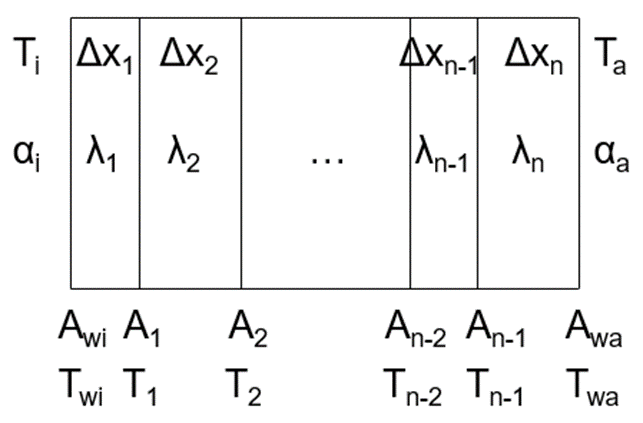
\includegraphics[width=\linewidth]{wand-serie}
		\caption{Serielle Wandschicht}
	\end{subfigure}
	\begin{subfigure}{0.28\textwidth}
		\centering
		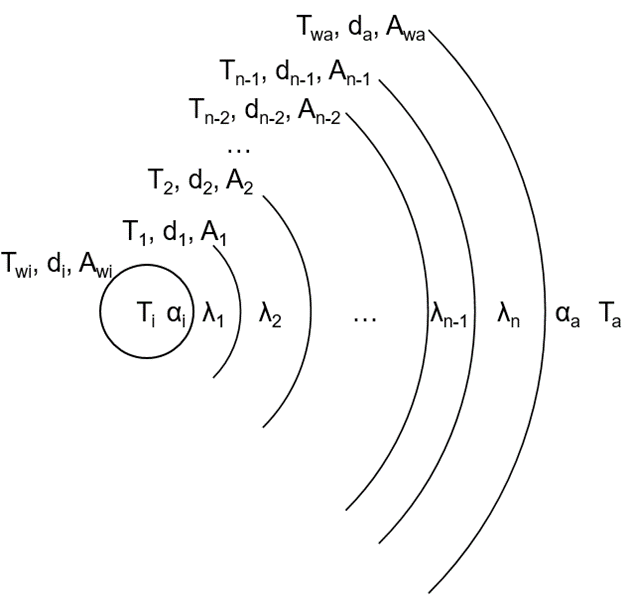
\includegraphics[width=\linewidth]{rohr-serie}
		\caption{Zylinder- und Kugelwand}
	\end{subfigure}
	\begin{subfigure}{0.45\textwidth}
		\centering
		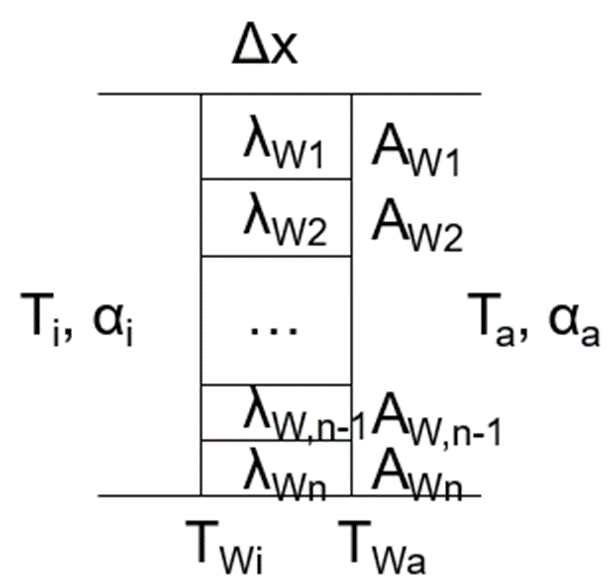
\includegraphics[width=0.4\linewidth]{wand-parallel}
		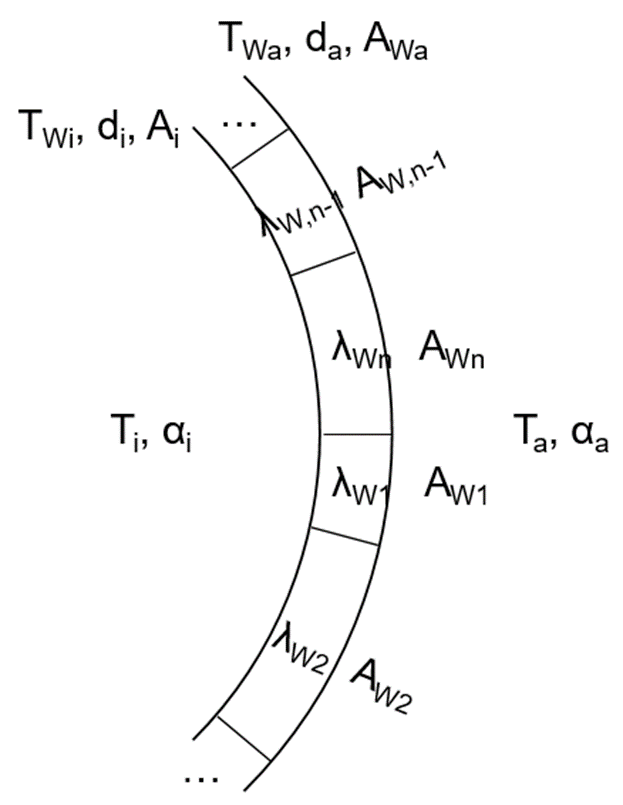
\includegraphics[width=0.5\linewidth]{rohr-parallel}
		\caption{Parallele Wandschichten}
	\end{subfigure}
\end{figure}

\clearpage

\subsection{Rippen}
	$ \eta_{Ri} = \dfrac{\dot{Q}_{Ri}}{\dot{Q}_{Ri,max}} = \dfrac{\tanh(m\ h)}{m\ h} $
		\qquad $ m = \sqrt{\dfrac{\alpha\ U}{\lambda_{Ri}\ A}} $
%		\qquad

	$ \dot{Q}_{Ri} = \lambda_{Ri}\ A_{Ri}\ \Delta T_0\ m \tanh(m\ h) $
		\qquad  $ \Delta T_{(x)} = T_{(x)} - T_u = \Delta T_0\, \dfrac{\cosh\left(m\ h \left(1- \frac{x}{h}\right)\right)}{\cosh(m\ h)} $
%		\qquad

	$ \dfrac{A_{w,mit}}{A_{w,ohne}} = 1 - \dfrac{A_{Ri}}{A_{w,ohne}} + \dfrac{A_{w,Ri}}{A_{w,ohne}} $
		\qquad\qquad $ \dfrac{\dot{Q}_{mit}}{\dot{Q}_{ohne}} = \dfrac{\alpha_{mit}}{\alpha_{ohne}} = 1 - \dfrac{A_{Ri}}{A_{w,ohne}}  + \dfrac{U_{Ri}}{A_{w,ohne}} \dfrac{\tanh(m\ h)}{m}$

\subsection{Transiente Wärmeleitung}
	$ a = \dfrac{\lambda}{\varrho\ c_p} $
		\quad $ \Four = \dfrac{a\ t}{s^2} $
		\quad $ \Biot = \dfrac{\alpha\ s}{\lambda} $
		\quad Platten: $ s = \dfrac{\Delta x}{2} $
		\quad Zylinder, Kugeln: $ s = \dfrac{d_a}{a} $
		\quad $\Theta = \dfrac{T - T_u}{T_0 - T_u}  $

\subsection{Konvektion}
	Durchströmung: $ L_{char} = d_h = \dfrac{4\ A}{U} $ \qquad Umströmung: $ L_{char} = L' = \dfrac{A_w}{U_{proj}}$

	\vskip 3pt
	$ \Reyn = \dfrac{c\ L_{char}}{\nu} $
		\quad $ \Pran = \dfrac{\nu}{a} = \dfrac{\mu\ c_p}{\lambda} = \dfrac{\delta}{\delta_T} $
		\quad $ \Rayl = \dfrac{g\ L_{char}\ \beta\ (T_w - T_{fl})}  {\nu\ a} $
		\quad $ \Nuss = \dfrac{\alpha\ L_{char}}{\lambda} = \dfrac{L_{char}}{\delta_T} $
		\quad $ \delta_T = \dfrac{\lambda}{\alpha} $

	\vskip 6pt
	$ \beta_{ideales~Gas} = \dfrac{1}{T_m} $
		\qquad Stoffwerte der WUE bei $ T_m = \dfrac{T_w + T_{fl}}{2} $


\subsection{Erzwungene Konvektion}
\subsubsection{Durchströmung}
	\setlength{\abovedisplayskip}{-20pt}
	\[ \arraycolsep=0.2em  \def\arraystretch{2}
	\begin{array}{lrll}
		\text{Laminar } \Reyn <2300: & \Nuss_{lam} & \multicolumn{2}{l}{ = \sqrt[3]{3,66^3 + 0,664^3\ \Pran \left(\Reyn \dfrac{d_h}{L}\right)^{\nicefrac{3}{2}}}}\\
		\text{Turbulent } \Reyn>10^4: &\Nuss_{turb} & \multicolumn{2}{l}{ = \dfrac{\nicefrac{ \zeta}{8}\Reyn\Pran}{1 + 12,7 \sqrt{\nicefrac{ \zeta}{8}} \left( \Pran^{\nicefrac{2}{3}} - 1\right)} \ f_1 \ f_2 } \\
		 \zeta = \left(1,8 \log(\Reyn) - 1,5\right)^{-2} & f_1 = 1 + \left(\dfrac{d_h}{L}\right)^{\nicefrac{2}{3}} & \quad f_{2,fl} = \left(\dfrac{\Pran}{\Pran_w}\right)^{0,11} &\quad f_{2,g} = \left(\dfrac{T}{T_w}\right)^{0,45} \\
		\text{Übergang: } \gamma = \dfrac{\Reyn-2300}{10000-2300} &\Nuss & \multicolumn{2}{l}{= (1-\gamma)\cdot \Nuss_{lam,\Reyn=2300} + \gamma\cdot \Nuss_{turb,\Reyn=10000}}\\
		\text{Ringspaltkorrektur: }&\Nuss_{Rs}& = \Nuss\ 0,86 \left(\dfrac{d_{aa}}{d_{ai}}\right)^{0,16}&
	\end{array} \]

\subsubsection{Umströmung}
	\setlength{\abovedisplayskip}{-20pt}
	\[ \arraycolsep=0.2em  \def\arraystretch{2}
	\begin{array}{lrrl}
		\text{Keine Anströmung: } & \Reyn<0,1:            & \Nuss_0      & = 0,1\ (\text{Platte}) \quad 0,3\ (\text{Zylinder}) \quad 2\ (\text{Kugel})                        \\
		\text{laminar: }          & 1<\Reyn<10^5:         & \Nuss_{lam}  & = 0,664 \sqrt[3]{\Pran}\sqrt{\Reyn}                                                                \\
		\text{Turbulent: }        & \num{5e5}<\Reyn<10^7: & \Nuss_{turb} & = \dfrac{0,037\ \Reyn^{0,8} \Pran}{1+ 2,443\ \Reyn^{-0,1} \left(\Pran^{\sfrac{2}{3}-1}\right)} f_3\\
		\multicolumn{2}{c}{f_{3,fl} =\left(\dfrac{\Pran}{\Pran_w}\right)^{0,25}} & \multicolumn{2}{c}{f_{2,g} = \left(\dfrac{T}{T_w}\right)^{0,121}}\\
		\text{Übergang: } & 10<\Reyn<10^7 & \Nuss& = \sqrt{\Nuss_{lam}^2 + \Nuss_{turb}^2}
	\end{array} \]

	\setlength{\abovedisplayskip}{-10pt}
	\[ \arraycolsep=1em  \def\arraystretch{1.5}
	\begin{array}{lll}
		\text{Schräg umströmter Zylinder:}
			& \text{Korrekturfaktor } f_5
			& \text{Längs umströmter Zylinder:} \\
		 \Nuss = \Nuss_{Zylinder,\ang{90}} \ f_5
			&  f_5 = \text{siehe Diag. nach \ref{sec:um-in-durch}}
			&  \Nuss =  \Nuss_{Platte}  \left(1+ 2,3 \dfrac{L}{d} \Reyn_L^{-0,5}\right)
	\end{array}\]

\subsubsection{Umströmung in Durchströmung} \label{sec:um-in-durch}
		\skipabove{-20pt}
		\[ \arraycolsep=1em  \def\arraystretch{1.7}
		\begin{array}{ll}
			\text{Hohlraumanteil:}                                                                                            & \multirow{3}{0.24\textwidth}{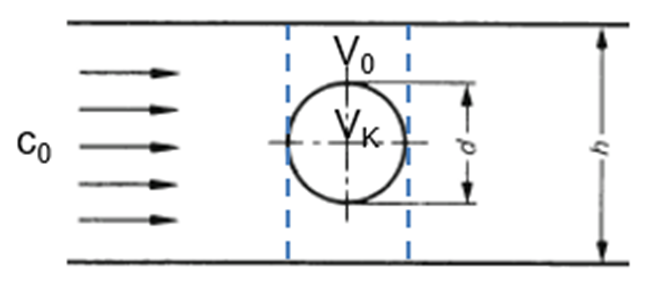
\includegraphics[width=\linewidth]{hohlraumanteil}} \\
			\varepsilon = 1- \dfrac{V_K}{V_0}  \qquad  c = \dfrac{c_0}{\varepsilon}                                           &                                                                                  \\
			\text{Rohrbündel:}                                                                                                & \multirow{9}{0.5\textwidth}{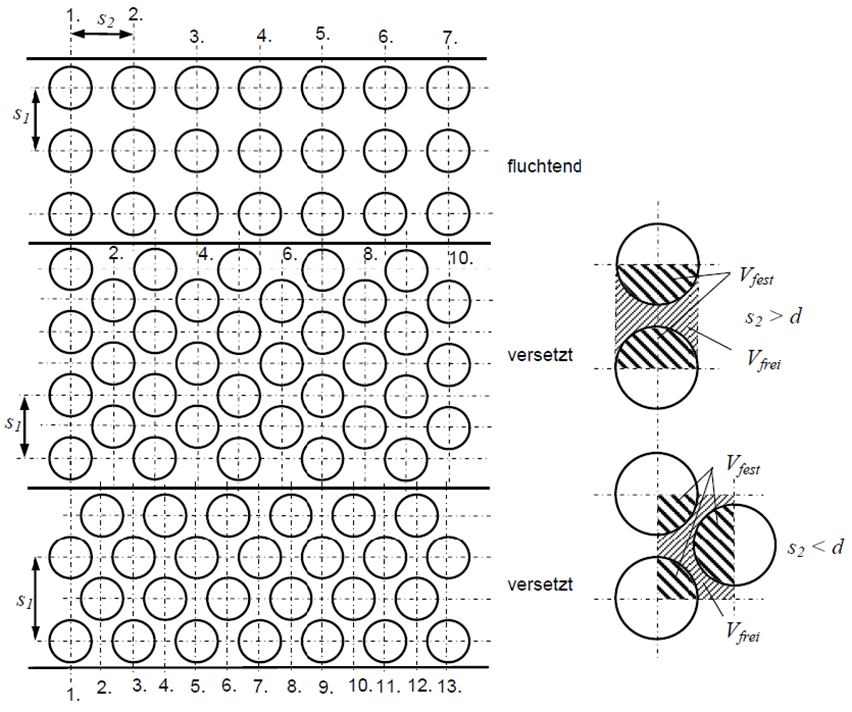
\includegraphics[width=\linewidth]{rohrbuendel}}     \\
			a = \dfrac{s_1}{d}  \qquad  b = \dfrac{s_2}{d}                                                                    &                                                                                  \\
			\Nuss_{B\ue ndel} = \Nuss_{einzel}\ f_A                                                                           &                                                                                  \\
			f_{A,fluchtend} = 1+ \dfrac{0,7 \left(\nicefrac{b}{a}-0,3\right)}{\varepsilon \left(\nicefrac{b}{a}+0,7\right)^2} &                                                                                  \\
			f_{A,versetzt} = 1 + \dfrac{2}{3\ b}                                                                              &                                                                                  \\
			n < 10: f_A = \dfrac{1+ (n-1) f_A}{n}                                                                             &                                                                                  \\
			\null                                                                                                             &                                                                                  \\
			\null                                                                                                             &                                                                                  \\
			\null                                                                                                             &
		\end{array} \]

	\begin{figure}[h]
		\centering
		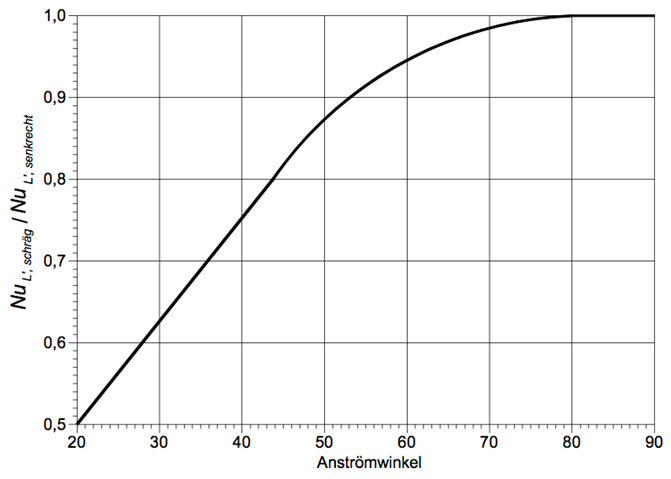
\includegraphics[width=9cm]{nusselt-winkel}
		\caption{Weil die Formel für $ f_5 $ noch fehlt}
	\end{figure}


\clearpage
\subsection{Freie Konvektion}
\subsubsection{Durchströmung}
	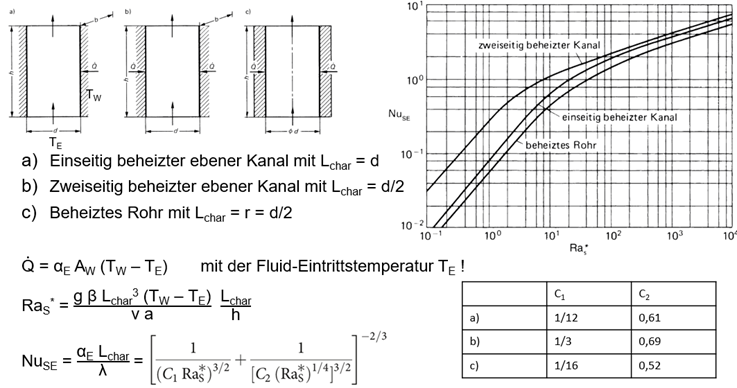
\includegraphics[width=0.9\textwidth]{FK-durchstroemung}

\subsubsection{Umströmung}
	Vertikale Wand: $ \Nuss = (0,825 + 0,387 \Rayl^{\sfrac{1}{6}} \ f_1) $
		\qquad\qquad $ f_1 = (1 + 0,671 \Pran^{\sfrac{-9}{16}}) ^{\sfrac{-8}{27}} $

	\vskip 0.2cm
	Geneigte Wand, Winkel $ \alpha $ zur Vertikalen: \qquad ohne Ablösung: $ \Rayl_{\alpha} = \Rayl\ \cos\alpha $

	\setlength{\abovedisplayskip}{-10pt}
	\[ \arraycolsep=0.7em  \def\arraystretch{1.4}
	\begin{array}{llc}
		\text{mit Ablösung:}
			& \Nuss = 0,56 \displaystyle\sqrt[4]{\Rayl_{krit}\, \cos\alpha} + 0,13 \left( \sqrt[3]{\Rayl} - \sqrt[3]{\Rayl_{krit}} \right)
			& \multirow{8}{5cm}{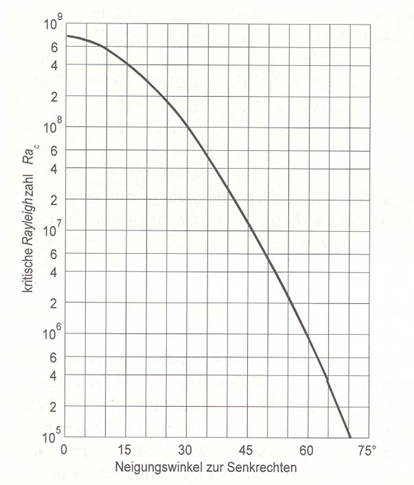
\includegraphics[width=\linewidth]{rayleigh-krit}} \\
		 & \Rayl_{krit} = 10^{(8,9 - 0,013\ \alpha - \num{5,95e-4}\ \alpha^2)} \text{ mit } \alpha \text{ in °} & \\
		 \multicolumn{2}{l}{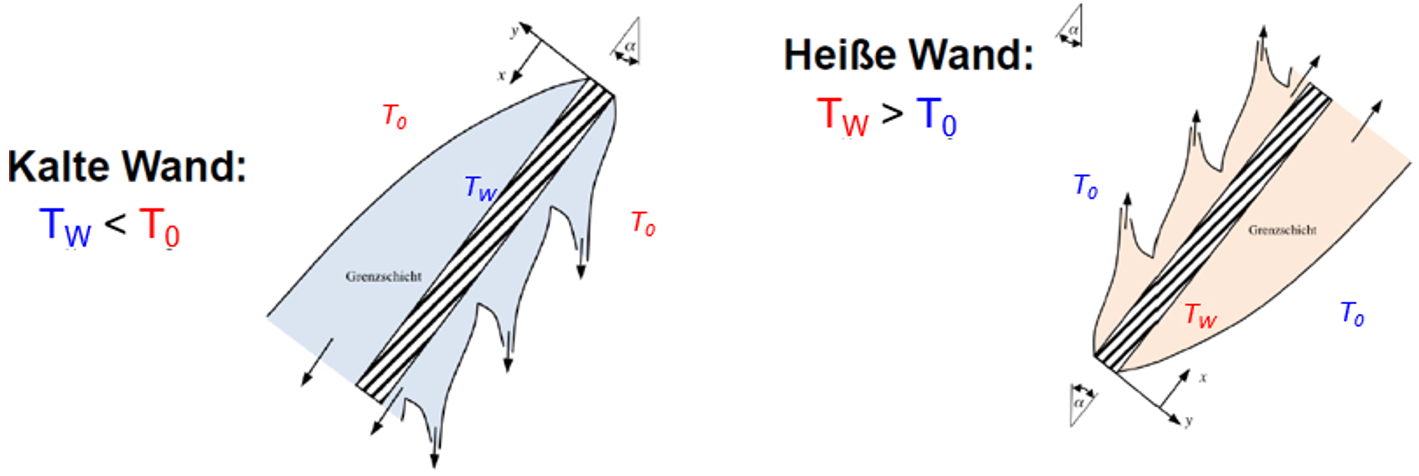
\includegraphics[width=11cm]{wand-abloesung}}
	\end{array}\]

	\setlength{\abovedisplayskip}{-15pt}
	\[ \arraycolsep=0.7em  \def\arraystretch{1.4}
	\begin{array}{lll}
		\text{Horizontale Wand:} &&\\
		 \Rayl\ f_2 \leq \num{7e4}: & \Nuss = 0,766 \displaystyle\sqrt[5]{\Rayl f_2} & f_2 = \left( 1+ 0,536 \Pran ^{\nicefrac{-11}{20}} \right) ^{\nicefrac{-20}{11}} \\
		 \Rayl\ f_2 > \num{7e4}: & \Nuss = 0,15 \displaystyle\sqrt[3]{\Rayl f_2} &\\
		 \text{Horizontaler Zylinder:} & \Nuss = \left(0,752 + 0,387 \sqrt[6]{\Rayl} f_3 \right)^2 & f_3 = \left( 1 + 0,721\Pran^{\nicefrac{-11}{20}}\right) ^{\nicefrac{-8}{27}} \\
		 \text{Kugel:} & \Nuss = 1 + 0,56\, \sqrt[4]{\dfrac{\Pran\Rayl}{0,846 + \Pran}}
	\end{array}\]

\subsubsection{Überlagerung mit erzwungener Konvektion}
	\[ \Nuss = \sqrt[3]{\Nuss_{erzwungen}^3 \pm \Nuss_{frei}^3} \qquad \text{+\dots gleichgerichtete, $-$\dots entgegen-gerichtete Mischkonvektion}\]

% \clearpage
\subsection{Wärmestrahlung zw. Oberflächen}
	\setlength{\abovedisplayskip}{-15pt}
	\[ \arraycolsep=0.4em  \def\arraystretch{1.7}
	\begin{array}{llc}
		\text{Strahlungsbilanz:}                          & a + r + t  =  1                                                                                                                                                                                     & \multirow{12}{2.6cm}{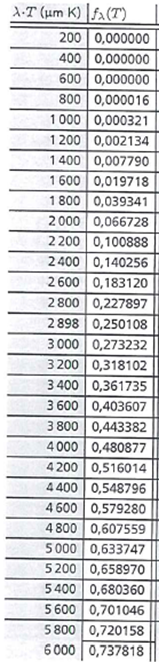
\includegraphics[width=\linewidth]{strahlung-tabelle-1}} \\
		\text{Planck'sches Gesetz:}                       & i_{s(\lambda,T)}  =  \dfrac{\Cone}{\lambda^5\left(\exp\left( \dfrac{\Ctwo}{\lambda\ T} \right) - 1\right)}                                                                                          &                                                                               \\
		\text{Mit: } \Cone=\qty{3,7418e-16}{\W\m\squared} & \Ctwo = \qty{1,438e-2}{\K\m\squared}                                                                                                                                                                &                                                                               \\
		\text{Wien'sches Gesetz:}                         & \lambda_{s,max}  =  \dfrac{2898}{T}  [\unit{\micro\m}]                                                                                                                                              &                                                                               \\
		\text{Stefan Boltzmann Gesetz: mit }\Cs  =  5,67  & \dot{q}_{s(T)}  =  \displaystyle\int_{\lambda = 0}^{\infty} i_{s(\lambda,T)} \ \dd \lambda  =  \Cs \left(\dfrac{T}{100}\right)^4                                                                    &                                                                               \\
		\text{Graue Bande:}                               & \dot{q}_{\lambda,s(T)}  =  \displaystyle\int_{\lambda = 0}^{\lambda} i_{s(\lambda,T)} \ \dd \lambda  = \varepsilon_{(\lambda)}\  f_{(\lambda,T)}\ \dot{q}_{s(T)}                                    &                                                                               \\
		\text{Kirchhoff'sches Gesetz:}                    & a = \varepsilon                                                                                                                                                                                     &                                                                               \\
		\text{Wärmestrom zw. zwei Flächen:}               & \dot{Q}_{12} = C_{12}\ A_{w1}\left[\left(\dfrac{T_1}{100}\right)^4 -\ \left( \dfrac{T_2}{100} \right) ^4\right]                                                                                     &                                                                               \\
		\multicolumn{2}{l}{ \text{Parallele Platten 1 und 2 mit N Platten ($\varepsilon_s$) dazwischen:}}                                                                                                                                                       &                                                                               \\
		\multicolumn{2}{l}{ \qquad C_{12} = \Cs\left[\dfrac{1}{\varepsilon_1} + \dfrac{1}{\varepsilon_2} -1 + N \left(\dfrac{2}{\varepsilon_s} - 1\right)\right] ^{-1}}                                                                                         &                                                                               \\
		\multicolumn{2}{l}{	\text{Konzentrische Zylinder/Kugelschalen (1 innen, 2 außen); N Schalen ($ \varepsilon_s $) dazwischen:}}                                                                                                                           &                                                                               \\
		\multicolumn{2}{l}{	\qquad C_{12} = \Cs\left[ \dfrac{1}{\varepsilon_1} + \dfrac{A_{w1}}{A_{w2}} \left(\dfrac{1}{\varepsilon_2} -1\right) + \left(\dfrac{2}{\varepsilon_s} - 1\right) \displaystyle\sum_{i=1}^{N} \dfrac{A_{w1}}{A_{wsi}} \right] ^{-1}}   & \multirow{12}{2.5cm}{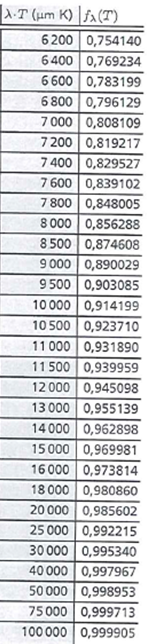
\includegraphics[width=\linewidth]{strahlung-tabelle-2}}     \\
		\text{Beliebig orientierte Flächen:}              & C_{12} = \Cs\dfrac{\varepsilon_1\ \varepsilon_2\ \varphi_{12}}{1-\left(1- \varepsilon_1\right)\left(1-\varepsilon_2\right) \varphi_{12}\ \varphi_{21}\ }                                            &    \\
		\text{\qquad mit Einstrahlzahlen:}                & \varphi_{12} = A_{w2} \dfrac{\cos{\beta_1}\cos{\beta_2}}{r^2\ \pi}   =  \varphi_{21} \dfrac{A_{w2}}{A_{w1}}                                                                                         &                                                                               \\
		\text{Umschlossener Körper 1:}                    & C_{12}  = \Cs \left[ \dfrac{1}{\varepsilon_1} +  \dfrac{A_{w1}}{A_{w2}} \left(\dfrac{1}{\varepsilon_2} - 1\right) \right]^{-1}                                                                      &                                                                               \\
		\text{\qquad wenn }A_{w2} \gg A_{w1}:             & C_{12} = \varepsilon_1\ \Cs                                                                                                                                                                         &                                                                               \\
		\text{Äquivalenter Wärmübergangskoeffizient:}     & \alpha_{Str} = \abs{\dfrac{{\dot{q}}_{Str}}{T_w - T_{fl}}}                                                                                                                                          &                                                                               \\
		\text{Emissionsgrad Umrechnung:}                  & \dfrac{\varepsilon}{\varepsilon_n}                                                                                                                                                                  &                                                                               \\
		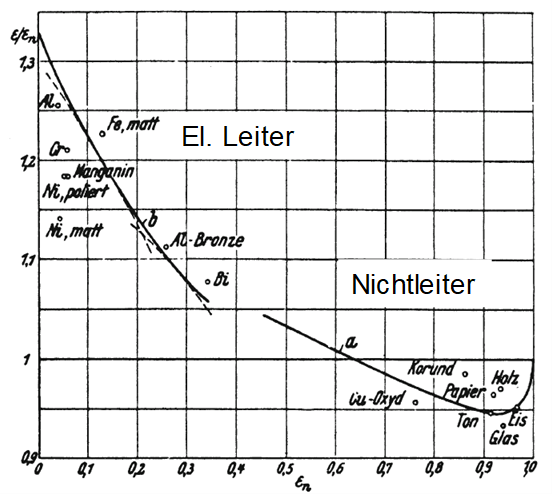
\includegraphics[width=7cm]{strahlung-epsilon}    & 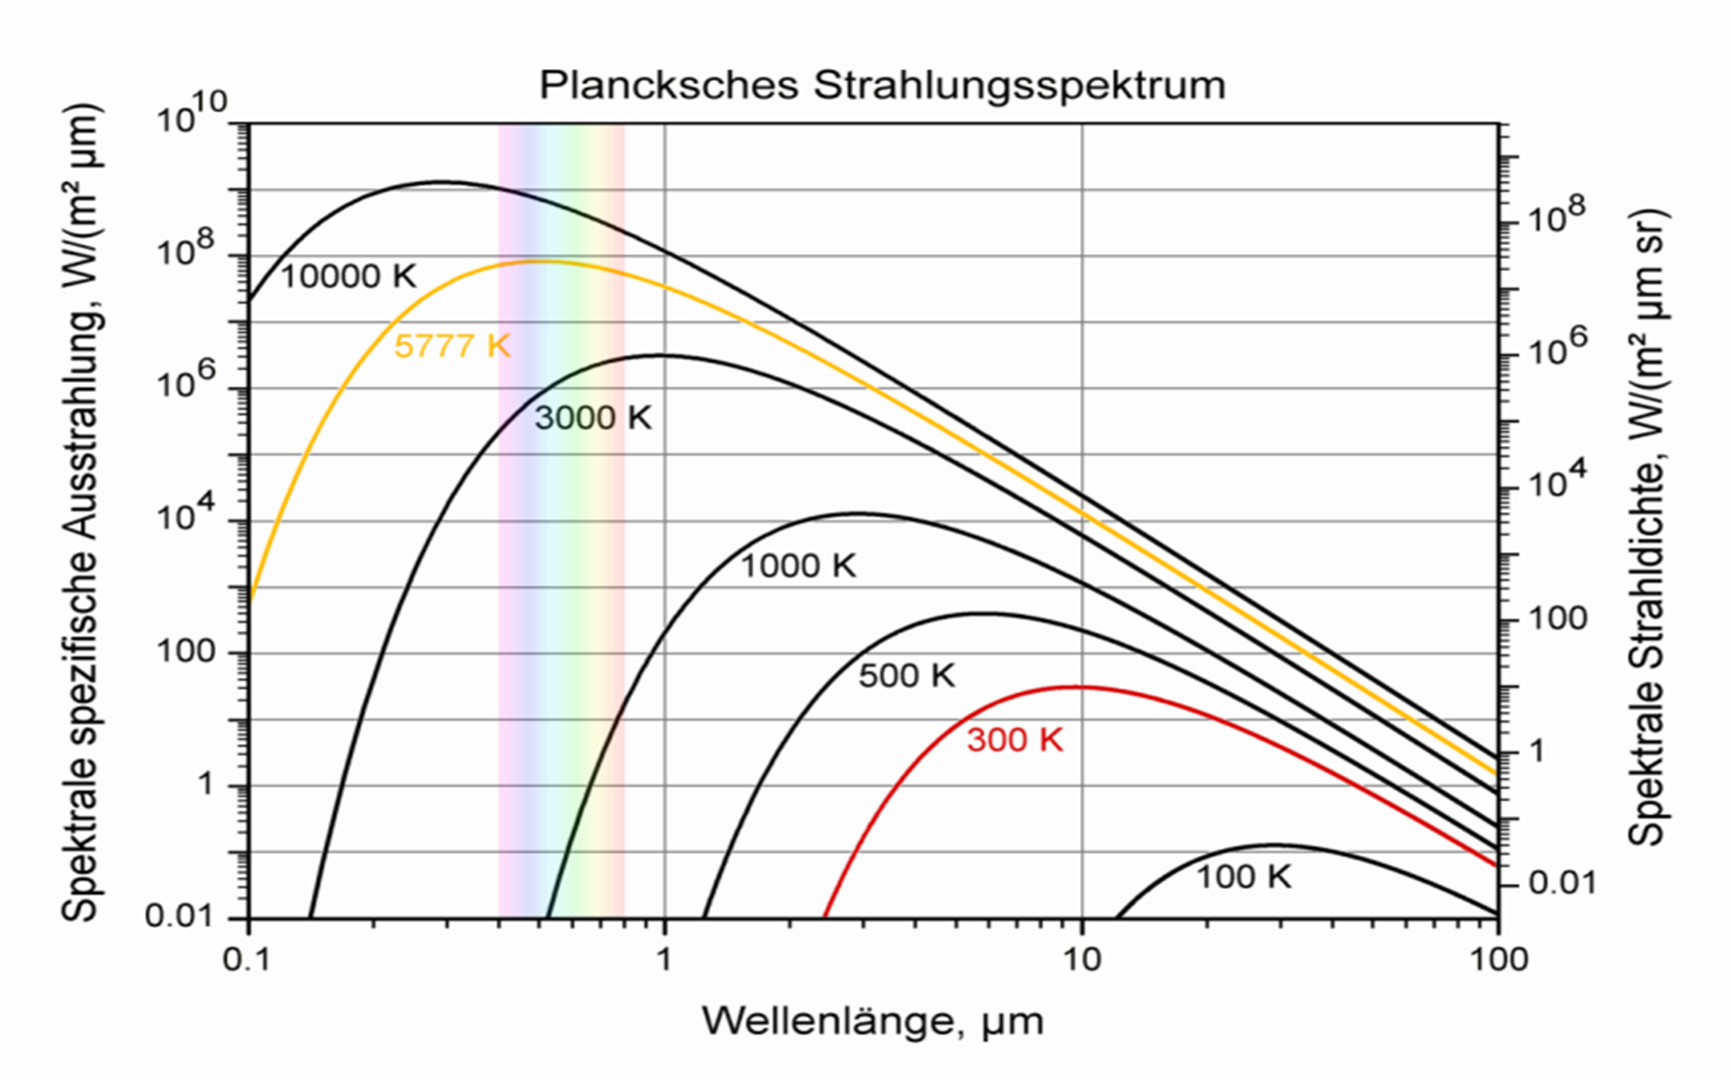
\includegraphics[width=7cm]{strahlung-planck}       &
	\end{array} \]



\subsection{Einseitig konstante Temperatur, Gleichstrom und Gegenstrom}
	\setlength{\abovedisplayskip}{-15pt}
	\[ \arraycolsep=0.4em  \def\arraystretch{1.7}
	\begin{array}{ll}
		\text{Übertragungseinheit}:          & N_i  =  \dfrac{k\ A_{wa}}{{\dot{m}}_i\ {cp}_i}                                                                                                                                                   \\
		\text{Mittlere Temperaturdifferenz:} & \Delta T  =  T_H - T_K  =  \dfrac{\Delta T_a - \Delta T_b} {\ln\left( \dfrac{\Delta T_a}{\Delta T_b}\right)} = \dfrac{\Delta T_b - \Delta T_a} {\ln\left( \dfrac{\Delta T_b}{\Delta T_a}\right)} \\
		\text{Mittlere Wandtemperaturen:}    & T_{wH}  =  T_H - \dfrac{k\ A_{wa}}{\alpha_H\ A_{wH}} \Delta T                                                                                                                                    \\
		                                     & T_{wK}  =  T_K + \dfrac{k\ A_{wa}}{\alpha_K\ A_{wK}} \Delta T
	\end{array} \]

\subsection{Einseitig konstante Temperatur} \label{sec:einseitig-konst-T}
	Übertragungseinheit: \qquad $ N  =  \dfrac{k\ A_{wa}}{\dot{m}\ cp}  =   \ln\left( \dfrac{\Delta T_a}{\Delta T_b} \right)  >  0 $

\subsection{Gleichstrom und Gegenstrom}
	Mittlere Temperaturen:	\qquad	$ T_H \cong \dfrac{T_{H1}+\ T_{H2}}{2}  \qquad T_K\cong \dfrac{T_{K1}+\ T_{K2}}{2} $

\subsection{Vorgangsweise Auslegung}
	\underline{Gegeben:} Geometrie außer Außen-Oberfläche, Einlass-Zustände beidseitig,

		\qquad \textbf{eine Ziel-Auslasstemperatur }

	\underline{Gesucht:} \textbf{Außenoberfläche der wärmeübertragenden Wand},

		\qquad davon abgeleitet Länge oder Rohranzahl etc.

	\begin{singlespace}
	\underline{Berechnung:}
		\begin{enumerate}
		\item Geometrie: Querschnittflächen, char. Abmessungen, etc.
		\item Wärmestrom, andere Auslasstemperatur, mittlere Temperaturdifferenz
		\item Annahme sinnvoller Wandtemperaturen auf beiden Seiten und zw. Wandschichten
		\begin{enumerate}
			\item Bei freier Konvektion, Wärmestrahlung:          \hfill 1. Annahme:	$ T_W \neq T_{fl}  $ \hspace{3cm} \null
			\item In Wärmeübertragern: nur erzwungene Konvektion, \hfill 1. Annahme:	$ T_W = T_{fl} $     \hspace{3cm} \null
		\end{enumerate}
		\item Stoffwerte beidseitig bei Mitteltemperatur zwischen Fluid und Wand
		\item Wand-, heißer -, kalter -, Gesamt-Widerstand, Wärmedurchgangskoeffizient
		\item Außenoberfläche der wärmeübertragenden Wand etc.
		\item Aktualisierung der Wandtemperaturen
		\item Übereinstimmung mit angenommenen Wandtemperaturen?
		\begin{enumerate}
			\item Ja $ \rightarrow $ OK
			\item Nein $ \rightarrow $ zurück zu 4.
		\end{enumerate}
		\end{enumerate}
	\end{singlespace}

\clearpage
\subsection{Vorgangsweise Betriebsnachrechnung}
	\underline{Gegeben:} \textbf{vollständige Geometrie}, Einlass-Zustände beidseitig

	\underline{Gesucht:} \textbf{Auslasstemperaturen beidseitig}

	\begin{singlespace}
		\underline{Berechnung:}
		\begin{enumerate}
			\item Vervollständigung geometrischer Daten (z.B. char. Abmessungen) und der Einlass-Zustände
			\item Annahme von k bzw. Übernahme von k aus Auslegung, iterative Aktualisierung:
		\end{enumerate}
	\end{singlespace}

\subsubsection{Einseitig konstante Temperatur }
	\[ \Delta T_2 = \Delta T_1\ \eul^{-N}   \qquad N\dots \text{ siehe \ref{sec:einseitig-konst-T}} \]

\subsubsection{Gleichstrom}
	\setlength{\abovedisplayshortskip}{-5pt}
	\[
		T_{H2} =  T_{H1} - (T_{H1} - T_{K1})\, \dfrac{\dot{W}_K}{\dot{W}_H + \dot{W}_K} \left(1- \eul^{-\mu\ k\ A_{wa}}\right)
		\hfil \mu = \dfrac{1}{\dot{W}_H} + \dfrac{1}{\dot{W}_K} \hfil
	\]
	\[
		T_{K2} =  T_{K1} - (T_{H1} - T_{K1})\, \dfrac{\dot{W}_K}{\dot{W}_H + \dot{W}_K} \left(1- \eul^{-\mu\ k\ A_{wa}}\right)
	\]

\subsubsection{Gegenstrom}
	\[
		\mu  = \abs{\dfrac{1}{\dot{W}_H} - \dfrac{1}{\dot{W}_K}}
	\]
	\[
		 T_{H2} =  T_{H1} - (T_{H1} - T_{K1})\, \dfrac{1-\ \eul^{-\mu\ k\ A_{wa}}}  {1- \dfrac{\dot{W}_H}{\dot{W}_K}\ \eul^{-\mu\ k\ A_{wa}}}
		 \qquad\qquad
		 T_{K2}  =  {T_{H1}} - (T_{H1} - T_{K1})\, \dfrac{1- \dfrac{\dot{W}_H}{\dot{W}_K}}  {1- \dfrac{\dot{W}_H}{\dot{W}_K}\ \eul^{-\mu\ k\ A_{wa}}}
	\]

\subsection{Rekuperatoren allgemein}
	\[
		P_H = \dfrac{T_{H1} - T_{H2}}{T_{H1} - T_{K1}}
		\qquad\qquad
		P_K = \dfrac{T_{K2} - T_{K1}}{T_{H1} - T_{K1}}
		\qquad\qquad
		\eta = \max(P_H,P_K)
	 \]
	 \[
	 	R_H = \dfrac{\dot{W}_H}{\dot{W}_K} = \dfrac{1}{R_K}
	 	\qquad\qquad
	 	\varTheta = \dfrac{T_H - T_K}{T_{H1} - T_{K1}} = F\ \varTheta_{Gegenstrom}
	 \]

	 $ F $ aus Betriebscharakteristik: $ f(P_H, \,N_H, \,N_K) = 0 $ oder $ f(P_H, \,N_H, \,R_H) = 0 $

\clearpage
\subsection{Regeneratoren}
	\[ \arraycolsep=0.1em  \def\arraystretch{1.6}
	\begin{array}{r l p{3em} r l}
		\Delta Q                                      & = \alpha_H\ A_w  \left(T_H - T_{wH}\right) \Delta t_H  &  & \Delta Q      & = \dfrac{\lambda_s}{\Delta s_w} A_w \left(T_{wH} - T_s\right) \Delta t_H                  \\
		\Delta Q                                      & = \alpha_K\ A_w  \left(T_{wK} - T_K\right) \Delta t_K  &  & \Delta Q      & = \dfrac{\lambda_s}{\Delta s_w} A_w \left(T_s - T_{wK}\right) \Delta t_K                  \\
		\dfrac{\Delta Q}{\Delta t_{H} + \Delta t_{K}} & = \dot{Q} = f\ k_0\ A _{w} \left( T_{H} - T_{K}\right) &  & T_{H} - T_{K} & = \dfrac{\Delta T_{a} - \Delta T_{b}}{\ln \left(\frac{\Delta T_{a}}{\Delta T_{b}}\right)} \\
		\Delta T_{a}                                  & = T_{H1} - T_{K2}                                      &  & \Delta T_{b}  & = T_{H2} - T_{K1} \\
		\dfrac{1}{k_0} & \multicolumn{4}{l}{= \left(\Delta t_{H} + \Delta t_{K}\right)  \left[\dfrac{1}{\alpha_{H}\ \Delta t_{H}} + \dfrac{1}{\alpha_{K}\ \Delta t_{K}} + \dfrac{\Delta s_{W}\ \Phi}{\lambda_{s}}  \left(\dfrac{1}{\Delta t_{H}}+\dfrac{1}{\Delta t_{K}}\right) \right]} \\
		 \text{mit } f,\ \Phi \text{ aus:}
	\end{array}\]


	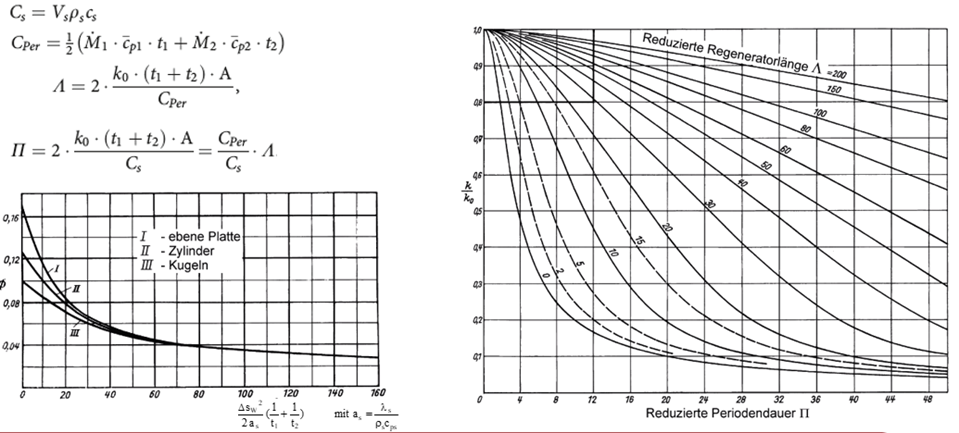
\includegraphics[width=0.95\textwidth]{regeneratoren}
\subsection{Gasstrahlung}
	Wärmestrom zw. heißem Gas (Flamme: $ \varepsilon_g,\ T_g $) einerseits und Wänden ($ T_w,\ \varepsilon_w $)

	und kaltem Gas an Wänden ($ T_w,\ a_g $) andererseits:

	\skipabove{0pt}
	\[ \dot{Q} = \dfrac{\varepsilon_w\ \Cs\ A_w}{1-\left(1-a_g\right)\ (1-\varepsilon_w)\ } \left[ \varepsilon_g \left( \dfrac{T_g}{100} \right)^4 - a_g \left( \dfrac{T_w}{100} \right)^4 \right] \]

	\[ \arraycolsep=0.1em  \def\arraystretch{1.3}
	\begin{array}{r l p{3em} r l}
		\varepsilon_g & = \varepsilon_{\ch{H2O}} + \varepsilon_{\ch{CO2}} - (\Delta\varepsilon)_g                           &  & a_g           & = a_{\ch{H2O}} + a_{\ch{CO2}} - (\Delta \varepsilon)_g                                              \\
		a _{\ch{H2O}} & = \varepsilon_{ \ch{H2O} ( Tw , p \ch{H2O}\ \sfrac{Tg}{Tw})}  \left(\dfrac{T_g}{T_w}\right) ^{0,45} &  & a _{\ch{CO2}} & = \varepsilon_{ \ch{CO2} ( Tw , p \ch{H2O}\ \sfrac{Tg}{Tw})}  \left(\dfrac{T_g}{T_w}\right) ^{0,65}
	\end{array}\]



	Emissionsgrade = Absorptionsgrade aus Diagrammen in Abhängigkeit von Temperatur, Druck, Partialdruck

	von \ch{CO2} bzw. \ch{H2O}, überlappenden Banden und gleichwertiger Schichtdicke $ s $

	\[ s= 0,9\, \dfrac{4\ V_g}{A_w} \]



